\chapter{Herramientas adicionales}\label{ap:HA}

\section{Recorte}

Haga click en \menu{Raster>Subset} y en la ventana que aparece elija la pestaña \menu{Geo Coordinates} (Figura \ref{fig:coordenadas}). Complete las coordenadas geográficas que contengan a la zona de interés y haga click en OK.

\begin{figure}[h!]
    \centering
    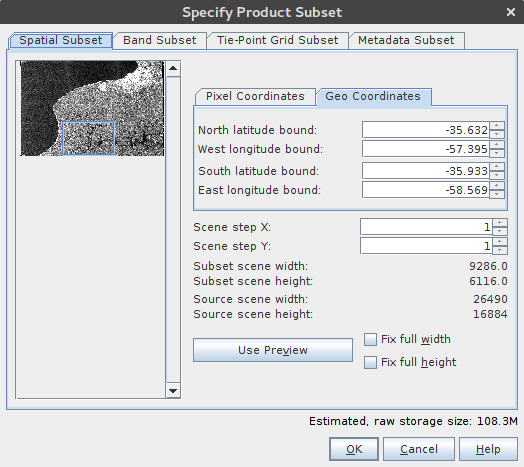
\includegraphics[scale=0.35]{fig:coordenadas.png}
    \caption{Subset espacial de una imagen en SNAP. Se realiza en este caso utilizando las coordenadas geográficas.}
    \label{fig:coordenadas}
\end{figure}

Obtendrá una nueva capa en el \emph{Product Explorer}. Para guardarlo haga click derecho sobre el y seleccione \menu{Save product as...}.

\section{Creación de vectores}

Cree un contenedor vectorial haciendo click en \menu{Vector>New Vector Data Container}. Nómbrelo \path{Urbano} (Figura \ref{fig:vector-cont}). Seleccione luego la herramienta \menu{Rectangle drawing tool} de la barra de herramienta y digitalice un rectángulo sobre una región. Para confirmar la geometría haga click fuera de ella.

\begin{figure}[h!]
    \centering
    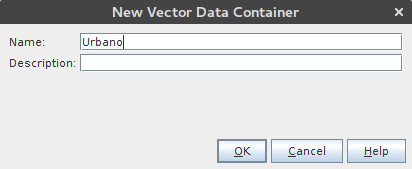
\includegraphics[scale=0.4]{fig:vector-cont.png}
    \caption{Herramienta de creación de contenedores vectoriales. Debe ser un nombre por cada uno y puede agregarse una descripción.}
    \label{fig:vector-cont}
\end{figure}

Puede crear varias geometrías dentro de un mismo vector o crear distintos contenedores vectoriales. Estos quedarán asociados al archivo y se guardarán haciendo click derecho sobre el nombre de la imagen y seleccionando \menu{Save product}.

\section{Estadística}

Haga click en \menu{Analysis>Statistics}. Haga click en el botón \menu{Refresh view}. El SNAP calculará la estadística.

\begin{figure}[ht!]
    \centering
    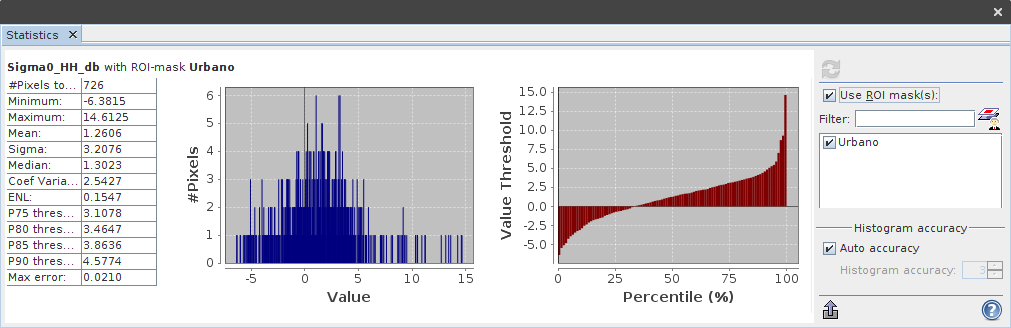
\includegraphics[scale=0.35]{fig:estadistica.png}
    \caption{Cálculo de parámetros estadísticos en SNAP. Es posible calcularlos sobre una región seleccionando \menu{Use ROI maks(s)} y luego la región de interés.}
    \label{fig:estadistica}
\end{figure}


Es posible calcular la estadística sobre una región. Para ello una vez abierta la ventana tilde la opción \texttt{Use ROI maks(s)} (Figura \ref{fig:estadistica}). Seleccione uno o más vectores. Haga click en el botón \menu{Refresh view}. El SNAP calculará la estadística sobre el vector. Puede hacerlo para varias regiones en simultáneo.

\section{Álgebra de bandas}

 Seleccione la herramienta \menu{Raster>Band maths...} (Figura \ref{fig:bm}).

 \begin{figure}[h!]
     \centering
     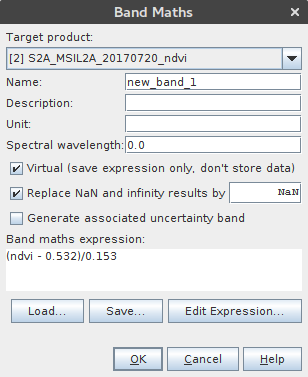
\includegraphics[scale=0.4]{fig:bm.png}
     \caption{Álgebra de bandas en el SNAP.}
     \label{fig:bm}
 \end{figure}

 En \emph{Band math expression:} puede escribir una expresión matemática utilizando el nombre de las bandas y distintos operadores.

 Es posible cambiar el nombre de la banda creada en la opción \emph{Name:} e incluir una descripción o unidades.

 {\bf Importante:} Por defecto se crea una banda virtual que calcula los valores \emph{al vuelo}. Para forzar el cálculo de la banda destilde la opción \emph{Virtual}.

 \section{Reproyección}

Para reproyectar una imagen vaya al menu \menu{Raster>Geometric>Reprojection}. Aquí deberá seleccionar la imagen de origen como input y la reproyectada como output. Para poder utilizar la imagen deberá elegir en \texttt{Reprojection parameters}, \texttt{Custom CRS} y allí seleccionar \texttt{Projection: Geographi Lat/Lon (WGS 84)} (Figura \ref{fig:reproj}).

 \begin{figure}[h!]
     \centering
     \subfloat[I/O Parameters]{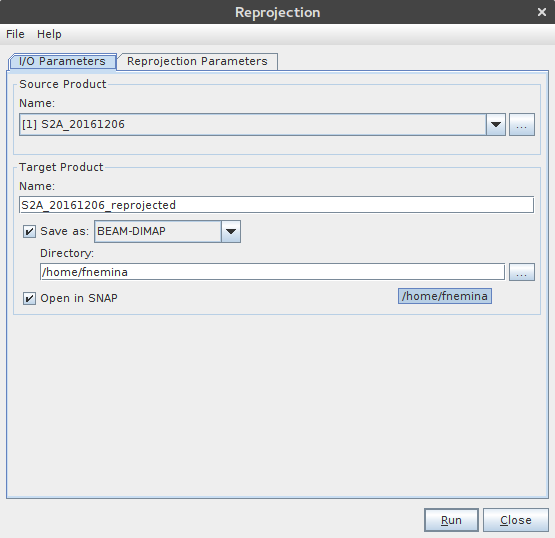
\includegraphics[width=0.35\textwidth]{fig:reproj1.png}}
     \hspace{1cm}
     \subfloat[Processing parameters]{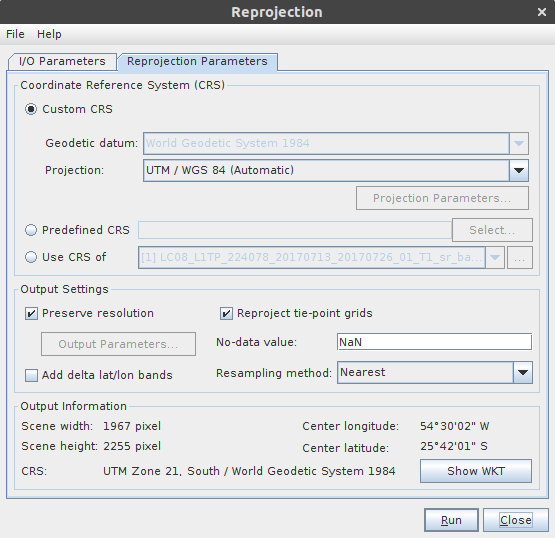
\includegraphics[width=0.35\textwidth]{fig:reproj2.png}}
     \caption{Herramienta de reproyección del SNAP. La imagen se proyecta en coordenadas geográficas.}
     \label{fig:reproj}
 \end{figure}
